\documentclass[a4paper,12pt]{article}   % 文檔類型為article
\usepackage{setspace}
\usepackage{fontspec}% 使用系统字体
\usepackage{xeCJK}    % 提供中文支持

% 设置中文正文字体为標楷體,你需要确保系统上有標楷體字体文件
\setCJKmainfont{標楷體}

%\onehalfspacing % 1.5 倍行距,與 Word 中的默認行距相同
%\pagestyle{empty}

\setmainfont{Times New Roman}
\fontsize{12pt}{\baselineskip}   % 設置字體大小為12pt,行距為單行


\usepackage{pdfpages}
\usepackage{enumitem}
\usepackage{fontspec}
\usepackage{authblk} 
\usepackage{titlesec}
\usepackage{amssymb}
\usepackage{graphicx}
\usepackage{titlesec}
\usepackage{float}

\titlespacing{\section}{0pt}{*2}{*1}
\titlespacing{\subsection}{0pt}{*2}{*1}
\titlespacing{\subsubsection}{0pt}{*2}{*1}

\usepackage{tabularx}
\usepackage{multirow}
%\usepackage{colortbl}
\usepackage{amsthm}
\usepackage{booktabs} % 用於漂亮的表格樣式


\usepackage{colortbl} % 用於表格顏色
\usepackage{xcolor}   % 用於文本顏色
\definecolor{lightgray}{gray}{0.9} % 自定義顏色
\newcommand{\xq}[1]{\textcolor{red}{#1}}

\pagestyle{plain}


\begin{document}
%\maketitle

\begin{center}
	{\fontsize{16pt}{12pt}\selectfont Semantic Segmentation on BCSS}
	
\end{center}

\hfill  B092040016 陳昱逢
	
	
\begin{center}
	Assignment 7
\end{center}

\section{U-Net architecture}
	Figure\ \ref{fig:unet} 呈現了 U-Net\ \cite{unet} 的架構圖,其部分想法類似於 ResNet 的殘差概念,更好地運用先前層的特徵,以達到好的分割效果。程式實作部分則是分每個節點都經過雙層的 convoluttion,再經由下採樣 (downsampling) 或是上採樣 (upsampling),其中上採樣經過一個類似於 fully convolution network (FCN) 中的反卷積 (deconvolution) 的概念,最後最淺層的 decoder 再經由最後一個卷積層輸出 mask。


\begin{figure}[htb]
  \vspace{0.1\baselineskip}  
  \centering  
  %\begin{center}
    \resizebox{0.9\textwidth}{!}{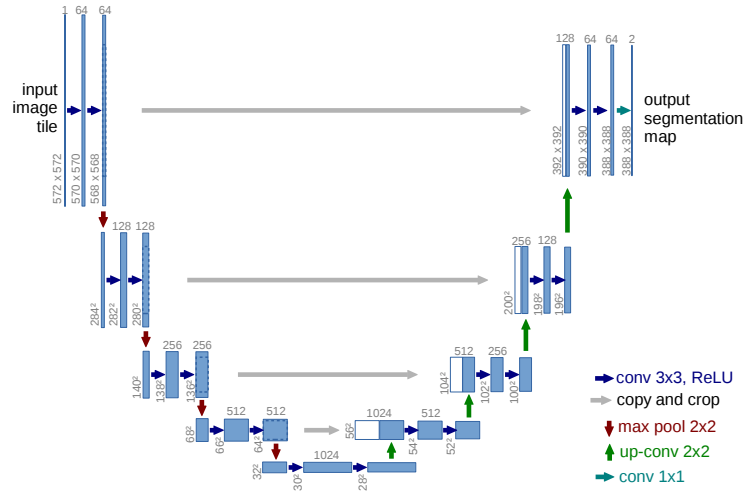
\includegraphics{fig/unet.png}}
    \caption{U-Net architecture\ \cite{unet}}
    \label{fig:unet}

  \vspace{0.1\baselineskip}
\end{figure}	

\section{增加模型的表現}

	為了增加模型的表現度,我採取了 U-Net++\ \cite{unetplus} 的類似想法,主要分成一個 donwsample 的 stream 以及很多 upsample 的 stream,考量實作方便以及運算資源,我只有實作四層的 U-Net++,以及簡化了一些殘差 (Residual) 的步驟,以確保我模型的通道累計是正確的。 相信此模型再結合了許多個upsample的stream後,模型的表現度可以再次被提高。 Figure\ \ref{fig:unetplus} 呈現了我的模型,想法來自於 U-Net++\ \cite{unetplus} 。

\begin{figure}[H]
  \vspace{0.1\baselineskip}  
  \centering  
  %\begin{center}
    \resizebox{0.5\textwidth}{!}{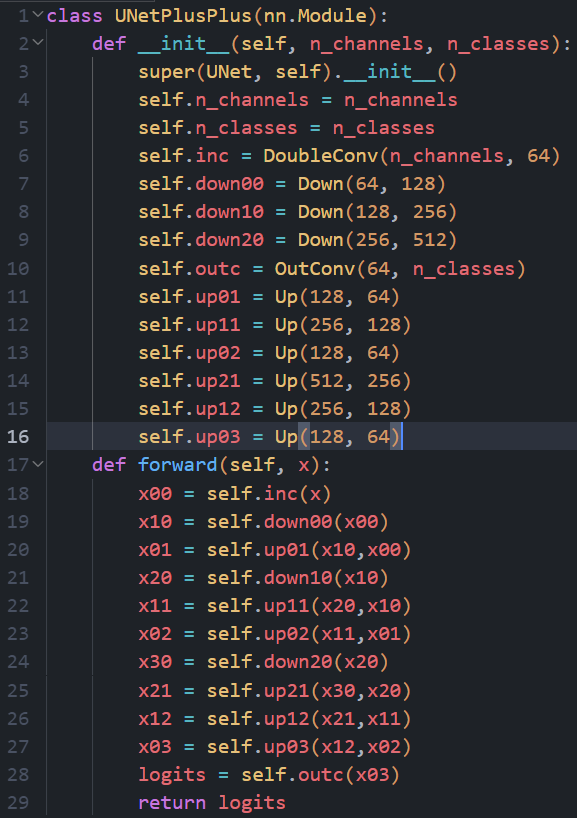
\includegraphics{fig/unetplus_code.png}}
    \caption{U-Net++ code}
    \label{fig:unetplus}
  %\end{center}
  \vspace{0.1\baselineskip}
\end{figure}	



\bibliographystyle{IEEEtran}
\bibliography{reference}



\end{document}